 \section{Introduction}

%What is the problem?
A key challenge in data-driven fields is the quality of training data. A fixed data collection budget can
provide a large amount of incomplete training data, or a smaller but cleaner dataset. Given a choice between these two options, which should we select and which factors should determine this decision? This question, while fundamental, is especially
relevant to modern machine learning, where vast amounts of unlabeled data is available. To exploit it without extensive hand-labeling, powerful techniques to exploit \emph{latent variable models}---in particular, latent variable \emph{method-of-moments}---have been developed. 

%where huge datasets are needed to train powerful models. The scale of these models has pushed against the limits of labeling budgets, motivating algorithmic generation of datasets. These can be generated from fitting a small sample of labeled data, or from unlabeled data with labels inferred via a \textit{latent variable graphical model}.

\begin{figure*}
    \centering
    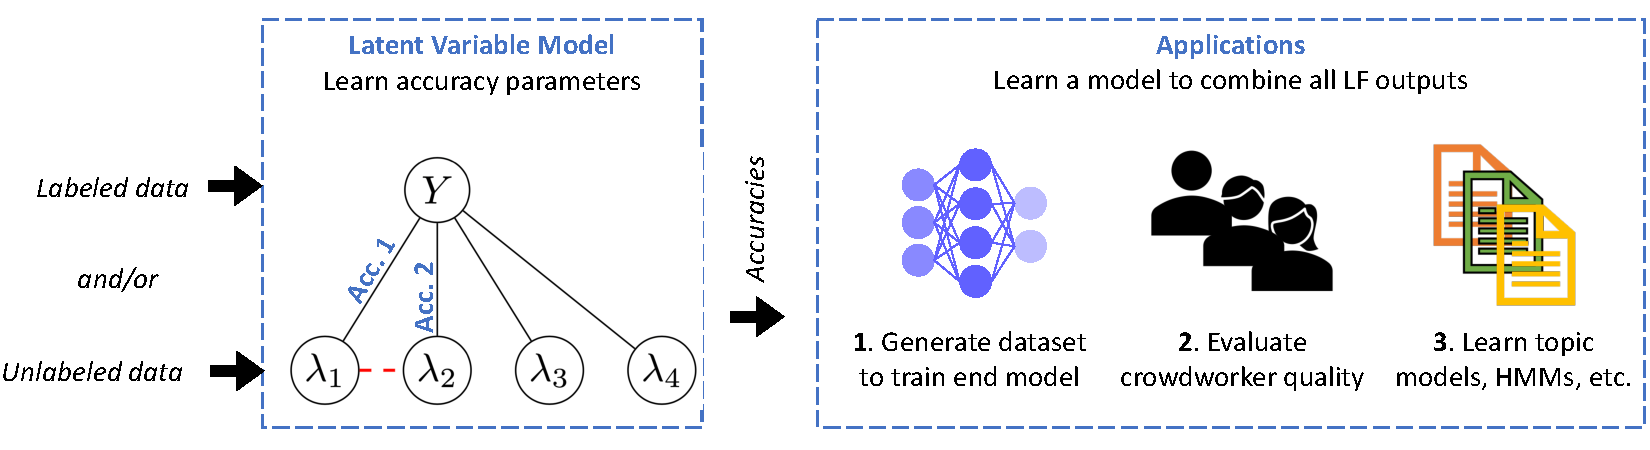
\includegraphics[width=.8\textwidth]{figures/maindiagram.pdf}
    %
    \caption{Latent variable methods (e.g., method-of-moments) can infer an unobserved variable ($Y$) by learning the accuracies of correlated sources ($\lf_1, \ldots, \lf_4$). This is done either from unlabeled data or directly from a small amount of labels; we seek a framework to explain the relative value of these choices. A major challenge are unmodeled dependencies between sources (red). Latent variable models have numerous applications.}
    \label{fig:systemdiagram}
\end{figure*}

Latent variable method-of-moments has been used to learn topic models \citep{anandkumar2014tensor}, parse trees \citep{Hsu12}, to evaluate crowdworkers \citep{joglekar2013evaluating}, and to generate training datasets \citep{Ratner19, fu2020fast}.
In these models, the outputs of sources---variables with some relation to the label---are observed and used to infer the latent variable. The core challenge is to learn the correlations (i.e., \emph{accuracies}) between the sources and the unobserved label variable, which parametrize the model used to generate labels.
%A small amount of labeled data can be used to directly estimate these correlations. 
Method-of-moments relies on decomposing multiple views of observed variables. When some labeled data is available, this setup also allows for the accuracy parameters to be directly estimated (Fig.~\ref{fig:systemdiagram}).
Therefore, given a limited budget, a principle for choosing between labeled and unlabeled data is crucial, motivating a theoretical framework to understand the relative value between them.

Unmodeled dependencies among sources---a form of model misspecification---are common and yield inconsistent accuracy estimates, which in turn yield poor inferred labels. This affects the value of data produced with latent variable methods, so misspecification must play a role in our framework. While the question of how to analyze misspecification has been studied in classical statistics, the focus is on estimators asymptotics \citep{kleijn2006, kleijn2012} or on impact on inference. Our main challenge, however, is to analyze and understand misspecification for both parameter estimation and label inference in the finite---and often small---sample setting.



We theoretically analyze the two alternatives in latent variable methods. In both cases, the output is a joint distribution forthe latent variable and observable sources. For the inputs, the choices are either $n_L$ labeled or $n_U$ unlabeled points (and the outputs of $m$ sources). We examine misspecification in the form of unmodeled pairwise dependencies, giving a generalization error analysis for method-of-moments latent variable model performance of the two alternatives. We present a bias-variance decomposition of the generalization error, which for both the labeled and unlabeled data cases consists of (i) irreducible error, (ii) variance, and (iii) bias due to model misspecification in inference. An important consequence is that for unlabeled data, we incur an additional (iv) error term due to incorrectly estimating accuracies that scales with the extent of misspecification, $\mathcal{O}(d/m)$ for $m$ sources and $d$ unmodeled dependencies among them. 

Next we turn to correcting this misspecification bias. In particular, a simple median approach is able to produce consistent estimators given that $d = o(m^2)$ and sufficient amounts of unlabeled data. Therefore, in certain cases, the standing bias $\mathcal{O}(d/m)$ from misspecification can be completely eliminated. This creates three scenarios to consider for our framework: well-specified (i.e. no unmodeled dependencies), misspecified, and corrected settings, depicted in Fig.~\ref{fig:biases}.

We give two applications of our theoretical framework for the three scenarios described above. First, we develop a criterion for choosing between labeled and unlabeled data called the \textit{data value ratio}, which is based on the relative minimum amount of labeled points needed to perform as well as a fixed amount of unlabeled points in terms of generalization error. For well-specified models, labeled data is only a constant factor more valuable than unlabeled, but for misspecified models the value grows linearly in the number of dependencies and unlabeled points. Furthermore, corrected (median-based) models are able to \emph{improve the value of unlabeled data}. Second, we combine the biased parameters learned from the unlabeled dataset with the unbiased ones learned from the labeled dataset---in certain cases outperforming either individually. We validate our  framework with synthetic experiments, verify the scaling of our generalization error and data value ratio, and the performance of the combined estimator across the three settings. 

An important real-world application of our results on latent-variable methods are weak supervision (WS) frameworks, in particular data programming \citep{Ratner16}, used in a huge range of products and systems across industry and academia. WS frameworks construct datasets without ground-truth annotations by using unlabeled points and distant or weak sources, such as heuristics~\citep{gupta2014improved}, external knowledge bases~\citep{mintz2009distant,craven:ismb99,takamatsu:acl12}, or noisy crowd-sourced labels~\citep{karger2011iterative,dawid1979maximum}. Data programming encompasses many such prior approaches, and has shown excellent results with the method-of-moments approach \citep{fu2020fast}. We perform real-world weak supervision experiments, where ground-truth source dependencies are not known, but sources are likely to be highly correlated. In several cases, we observe that the relative value of labeled data is large, but can be reduced via our median approach. \todo{Number here}. This suggests that our theoretical explanation of the effects of misspecification can account for some of the behavior of models on real data.

%A key challenge in data-driven fields is the quality of data. A fixed data collection budget can provide a large amount of noisy or incomplete data, or a smaller but cleaner dataset. Given a choice between these two options, which should we select and which factors should determine this decision? This question, while fundamental, is especially relevant to modern machine learning, where huge datasets are needed to train powerful models. The scale of these models has pushed against the limits of labeling budgets, motivating the use of generative \emph{latent-variable} models that obviate hand-labeling each point.

%Instead, in latent variable methods, the outputs of alternative sources or views---variables that have some relationship to the label---are observed and are used to estimate the value of the latent variable. The core technical challenge is to learn the correlations (i.e., \emph{accuracies}) between the alternative sources and the unobserved label variable. A small amount of labeled data can be used to directly estimate these correlations. They can also be obtained without access to any labels via approaches such as multi-view \emph{latent-variable method-of-moments}---the technique we study in this paper. Both approaches stand to benefit from additional datapoints. Given a limited budget, a principle for choosing between these two is crucial, motivating the need for a theoretical framework to understand the relative value of labeled versus unlabeled data.

%Unmodeled dependencies between these variables---a form of model misspecification---yields inconsistent correlation estimates, producing poor-quality output labels. In turn, this affects the value of data produced with latent variable methods. A principle for choosing between these two is crucial, motivating the need for a theoretical framework to understand the relative value of labeled versus weakly-labeled data.

%We theoretically analyze the two alternatives in latent variable methods. In both cases, the outputs are a set of accuracy parameters, but for the inputs, the choices are either a set of $n_L$ labeled points or a set of $n_U$ unlabeled points and the outputs of $m$ observable sources. We focus on the method-of-moments estimator as our latent-variable method. We examine misspecification in the form of unmodeled pairwise dependencies and incorporate this into a generalization error analysis for latent variable model performance of the two alternatives---the main component of our theoretical framework. We present a bias-variance decomposition of the generalization error, which for both the labeled and unlabeled data cases consists of (i) irreducible error, (ii) variance, and (iii) bias due to model misspecification in statistical inference. An important consequence is that for unlabeled data, we incur an additional (iv) error term due to incorrectly estimating accuracies that scales with the extent of misspecification, $\mathcal{O}(d/m)$ for $m$ sources and $d$ unmodeled dependencies among them. 

%We next turn to correcting this misspecification bias in method-of-moments latent variable estimators. In particular, a simple median approach is able to produce consistent estimators given $d = o(m^2)$ and sufficient amounts of unlabeled data. Therefore, in certain cases, the standing bias $\mathcal{O}(d/m)$ from misspecification can be completely eliminated theoretically. This creates three scenarios to consider our framework in: well-specified (i.e. no unmodeled dependencies), misspecified, and corrected settings, depicted in Figure \ref{fig:biases}.  


%We then present two applications of our theoretical framework for the three scenarios described above. First, we develop a criterion for choosing between labeled and unlabeled data called the \textit{data value ratio}, which is based on the relative minimum amount of labeled points needed to perform as well as a fixed amount of unlabeled points in terms of generalization error. For well-specified models, labeled data is only constant factor more valuable than unlabeled data, but for misspecified models the value grows linearly in the number of dependencies and unlabeled points. Furthermore, corrected (median-based) models are able to \emph{improve the value of unlabeled data}. Second, we discuss how combining the biased parameters learned from the unlabeled dataset with the unbiased ones learned from the labeled dataset can outperform either individually. We validate our theoretical framework with  synthetic experiments, verify the scaling of our generalization error, the scaling of the data value ratio, and the performance of the combined estimator across the three settings. 

%An important real-world application of our results on latent-variable methods are weak supervision (WS) frameworks, in particular data programming \citep{Ratner16}, used in a huge range of products and systems across industry and academia. WS frameworks construct datasets without ground-truth annotations by using unlabeled points and distant or weak sources, such as heuristics~\citep{gupta2014improved}, external knowledge bases~\citep{mintz2009distant,craven:ismb99,takamatsu:acl12}, or noisy crowd-sourced labels~\citep{karger2011iterative,dawid1979maximum}. Data programming encompasses many such prior approaches, and has shown excellent results with the method-of-moments approach \citep{fu2020fast}. We perform real-world weak supervision experiments, where ground-truth source dependencies are not known, but sources are likely to be highly correlated. In several cases, we observe that the relative value of labeled data is large, but can be reduced via our median approach. \todo{Number here}. This suggests that our theoretical explanation of the effects of misspecification can account for some of the behavior of models on real data.



%, so misspecification must be theoretically factored into our framework. While the question of how to analyze misspecification has been studied in classical statistical works, they primarily focus on asymptotic behavior of estimators~\citep{kleijn2006, kleijn2012}. Our main challenge, however, is to handle the finite---and often very small---sample setting since we wish to compare datasets practically. 


%Given a choice between these two options, which should we select and which factors should determine this decision? This question, while fundamental, is especially relevant to an important area of machine learning---weakly-supervised learning---where such datasets are used to train an intermediate model that outputs a larger, de-noised dataset to be used downstream (e.g., to train a data-hungry deep model).
%


%Why is it interesting and important?
%Such techniques are motivated by the scale of modern ML, which has pushed against the limits of budgets for building hand-labeled datasets. Weak supervision (WS) frameworks, in particular data programming \citep{Ratner16}---used in a huge range of products and systems across industry and academia---construct datasets without ground-truth annotations by using unlabeled points and distant or weak sources, such as heuristics~\citep{gupta2014improved}, external knowledge bases~\citep{mintz2009distant,craven:ismb99,takamatsu:acl12}, or noisy crowd-sourced labels~\citep{karger2011iterative,dawid1979maximum}. Data programming encompasses many approaches and has the advantage of being expressed in terms of classical models, allowing for theoretical analysis. Such approaches benefit from adding more labeled data and/or  \textit{weakly-labeled} data, i.e., unlabeled points in the context of weak sources. A principle for choosing between these two is crucial, motivating the need for a theoretical framework to understand the relative value of labeled versus weakly-labeled data.

% Why is it hard? (E.g., why do naive approaches fail?)



%The core technical challenge in WS is to learn the accuracies of weakly-labeled data sources. A latent variable statistical model whose parameters include the accuracies is fit to the weakly-labeled data and then used to output de-noised labels on the data. Unmodeled dependencies between sources---a form of model misspecification---yields inconsistent source accuracy estimates, producing poor-quality output labels. In turn, this affects the value of weakly-labeled data, so misspecification must be theoretically factored into our framework. While the question of how to analyze misspecification has been studied in classical statistical works, they primarily focus on asymptotic behavior of estimators~\citep{kleijn2006, kleijn2012}. Our main challenge, however, is to handle the finite---and often very small---sample setting since we wish to compare datasets practically. 

%We theoretically analyze the two alternatives in weak supervision pipelines. In both cases, the outputs are a set of accuracy parameters, but for the inputs, the choices are either a set of $n_L$ labeled points or a set of $n_U$ weakly-labeled points from $m$ weak sources. We examine misspecification in the form of unmodeled pairwise dependencies and incorporate this into a generalization error analysis for WS model performance of the two alternatives---the main component of our theoretical framework. We present a bias-variance decomposition of the generalization error, which for both the labeled and weakly-labeled data cases consists of (i) irreducible error, (ii) variance, and (iii) bias due to model misspecification in statistical inference. An important consequence is that for weakly-labeled data, we incur an additional (iv) error term due to incorrectly estimating accuracies that scales with the extent of misspecification, $\mathcal{O}(d/m)$ for $m$ sources and $d$ unmodeled dependencies among them. 



%We next turn to correcting this misspecification bias. In particular, a simple median approach is able to produce consistent estimators given $d = o(m^2)$ and sufficient amounts of weakly-labeled data, and this finding also broadly applies to other method-of-moments algorithms that exploit multiple, conditionally-independent views of latent variables. Therefore, the standing bias $\mathcal{O}(d/m)$ from misspecification can be completely eliminated theoretically. This creates three scenarios to consider our framework in: well-specified (i.e. no unmodeled dependencies), misspecified, and corrected settings, depicted in Figure \ref{fig:biases}.  

%We then present two applications of our theoretical framework for the three scenarios described above. First, we develop a criterion for choosing between labeled and weakly labeled data called the \textit{data value ratio}, which is based on the relative minimum amount of labeled points needed to perform as well as a fixed amount of unlabeled points in terms of generalization error. For well-specified models, labeled data is only constant factor more valuable than unlabeled data, but for misspecified models the value grows linearly in the number of dependencies and unlabeled points. Furthermore, corrected (median-based) models are able to \emph{reduce the value of labeled data}. Second, we discuss how combining the biased parameters learned from the unlabeled dataset with the unbiased ones learned from the labeled dataset can outperform either individually.

%What are the key components of my approach and results? Also include any specific limitations.
%We validate our theoretical framework with  synthetic experiments, verify the scaling of our generalization error, the scaling of the data value ratio, and the performance of the combined estimator across the three settings. In addition, we collect real-world experimental data, where ground-truth dependencies are not known, but sources are likely to be highly correlated. In several cases, we observe that the relative value of labeled data is large, but can be reduced via our median approach. This suggests that our theoretical explanation of the effects of misspecification can account for some of the behavior of models on real data.



%%%%%%%%%%%%%%%%%%%%%%%%%%%%%%%%% OLD (10/14)


%A key challenge in data-driven fields is the quality
%of training data. A fixed data collection budget can
%provide a large amount of noisy or incomplete training data, or a smaller but cleaner dataset. Given a
%choice between these two options, which should we
%select and which factors should determine this decision? This question, while fundamental, is especially
%relevant to an important area of machine learning—
%weakly-supervised learning—where such datasets are
%used to train an intermediate model that outputs a
%larger, de-noised dataset to be used downstream (e.g.,
%to train a data-hungry deep model).

%Such techniques are motivated by the scale of modern ML, which has pushed against the limits of budgets for building hand-labeled datasets. Weak supervision (WS) frameworks, in particular data programming (Ratner et al., 2016)—used in a huge range of
%products and systems across industry and academia—
%construct datasets without ground-truth annotations
%by using unlabeled points and distant or weak sources,
%such as heuristics (Gupta and Manning, 2014), external knowledge bases (Mintz et al., 2009; Craven
%and Kumlien, 1999; Takamatsu et al., 2012), or noisy
%crowd-sourced labels (Karger et al., 2011; Dawid and
%Skene, 1979). Data programming encompasses many
%approaches and has the advantage of being expressed
%in terms of classical models, allowing for theoretical
%analysis. Such approaches benefit from adding more
%labeled data and/or weakly-labeled data, i.e., unlabeled
%points in the context of weak sources. A principle for
%choosing between these two is crucial, motivating the
%need for a theoretical framework to understand the
%relative value of labeled versus weakly-labeled data.


%The core technical challenge in WS is to learn the accuracies of weakly-labeled data sources. A latent variable statistical model whose parameters include the
%accuracies is fit to the weakly-labeled data and then
%used to output de-noised labels on the data. Unmodeled dependencies between sources—a form of model
%misspecification—yields inconsistent source accuracy
%estimates, producing poor-quality output labels. In
%turn, this affects the value of weakly-labeled data, so
%misspecification must be theoretically factored into our
%framework. While the question of how to analyze misspecification has been studied in classical statistical
%works, they primarily focus on asymptotic behavior
%of estimators (Kleijn and van der Vaart, 2006, 2012).
%Our main challenge, however, is to handle the finite—
%and often very small—sample setting since we wish to
%compare datasets practically.


%We theoretically analyze the two alternatives in weak
%supervision pipelines. In both cases, the outputs are
%a set of accuracy parameters, but for the inputs, the
%choices are either a set of $n_L$ labeled points or a set of
%$n_U$ weakly-labeled points from m weak sources. We
%examine misspecification in the form of unmodeled
%pairwise dependencies and incorporate this into a gen-
%eralization error analysis for WS model performance
%of the two alternatives—the main component of our
%theoretical framework. We present a bias-variance de-
%composition of the generalization error, which for both
%the labeled and weakly-labeled data cases consists of
%(i) irreducible error, (ii) variance, and (iii) bias due to
%model misspecification in statistical inference. An im-
%portant consequence is that for weakly-labeled data,
%we incur an additional (iv) error term due to incor-
%rectly estimating accuracies that scales with the ex-
%tent of misspecification, $\mathcal{O}(d/m)$ for $m$ sources and $d$
%unmodeled dependencies among them.
%We next turn to correcting this misspecification
%bias. In particular, a simple median approach is
%able to produce consistent estimators given $d = o(m^2)$ and sufficient amounts of weakly-labeled data,
%and this finding also broadly applies to other
%method-of-moments algorithms that exploit multiple,
%conditionally-independent views of latent variables.
%Therefore, the standing bias $\mathcal{O}(d/m)$ from misspecification can be completely eliminated theoretically.
%This creates three scenarios to consider our framework
%in: well-specified (i.e. no unmodeled dependencies),
%misspecified, and corrected settings, depicted in Fig-ure 1.


%We then present two applications of our theoretical
%framework for the three scenarios described above.
%First, we develop a criterion for choosing between la-
%beled and weakly labeled data called the data value
%ratio, which is based on the relative minimum amount
%of labeled points needed to perform as well as a fixed
%amount of unlabeled points in terms of generalization
%error. For well-specified models, labeled data is only
%constant factor more valuable than unlabeled data, but
%for misspecified models the value grows linearly in the
%number of dependencies and unlabeled points. Furthermore, corrected (median-based) models are able
%to reduce the value of labeled data. Second, we discuss
%how combining the biased parameters learned from the
%unlabeled dataset with the unbiased ones learned from
%the labeled dataset can outperform either individually.
%We validate our theoretical framework with synthetic
%experiments, verify the scaling of our generalization error, the scaling of the data value ratio, and the performance of the combined estimator across the three set-
%tings. In addition, we collect real-world experimental
%data, where ground-truth dependencies are not known,
%but sources are likely to be highly correlated. In several cases, we observe that the relative value of labeled
%data is large, but can be reduced via our median approach. This suggests that our theoretical explanation
%of the effects of misspecification can account for some
%of the behavior of models on real data.